\documentclass[a4paper,12pt]{article}
\usepackage[utf8]{inputenc}
\usepackage[a4paper]{geometry}
\usepackage{graphicx, subfigure}
\usepackage{url}
\usepackage[superscript]{cite}
\usepackage{wrapfig}
\renewcommand\thesection{\arabic{section}}
\usepackage{listings}
\usepackage{url}




\begin{document}

%------- Introduction begins -----------------------
\section{Introduction}
More than half of elements heavier than iron, including platinum and gold, are thought to be the result of the astrophysical rapid neutron capture process (r-process) of nucleosynthesis. Due to the underlying physics, the r-process carves a path through highly neutron rich regions of the nuclear chart, far from stability. The exact path remains a mystery, as most of the nuclei in question have never been observed (see figure~\ref{fig:unknownChart}), and there is little experimental data \cite{cowan}{}. By determining the properties of these exotic nuclei, for instance their masses, the path of the r-process can be better constrained. Without reliable experimental data, r-process models have, as yet, been unable to reproduce observed elemental abundances.

\begin{figure}[h]
\label{fig:unknownChart}
\centering
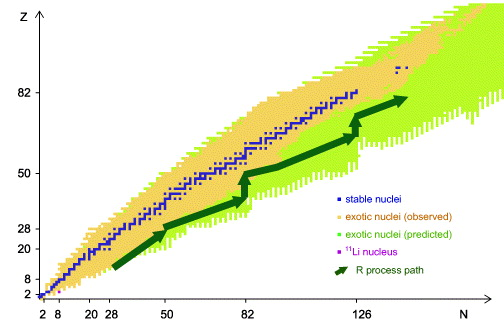
\includegraphics[height=10cm]{nuclearChart}
\caption{A nuclear chart of proton number against neutron number, with stable and exotic nuclei shaded, along with the path of the r-process. The r-process path traverses the extremely unstable, neutron rich region of the nuclear chart\cite{otsuka}{}.}
\end{figure}


Here, data from photon-induced multi-proton knockout experiments is analysed to determine the properties of highly neutron rich nuclei, far from stability. Such exotic nuclei are possible r-process path candidates. The data come from experiments by the A2 Collaboration using the Crystal Ball detector, currently situated at the Mainz Microtron (MAMI) in Germany. By studying reactions where relatively large numbers of protons have been knocked out, and utilising experiments that have used heavier targets than usual, such as lead, it is hoped that current knowledge can be improved upon.  

A further uncertainty of the r-process is its exact astrophysical site. Although it is likely that supernovae are the answer, in part due to the high flux of neutrons present, this has yet to be definitively confirmed \cite{thielemann}{}. More precise experimental data on the relevant nuclei involved, as well as a better idea of which nuclei are relevant, may lead to further insights into the nature of the r-process.


%More like background.
\section{Background}
\subsection{R-Process}
For over half a century, it has been known that virtually all of the elements beyond Helium that are found in nature are the product of nuclear reactions involving stars. Nucleosynthesis of successively heavier nuclei proceeds via nuclear fusion until iron, the nucleus with the highest binding energy per nucleon. Beyond this point, the coulombic repulsion arising from nuclear protons means that charged particle induced reactions reduces rapidly become unfeasible at stellar temperatures\cite{iliadis}{}. The iron peak also marks the turning point where nuclear fusion becomes endothermic. Elements heavier than iron are therefore synthesised mainly by a combined process of neutron capture, disintegration, and beta-decay\cite{b2fh}{}. The neutron capture cross section at typical stellar temperatures is usually high, with the high Coulomb barrier being irrelevant for neutrally charged particles\cite{iliadis}{}. 

Neutron capture is accompanied by the emission of a photon, as demonstrated by (\ref{eq:nCapture}).

\begin{equation}
\label{eq:nCapture}
N(Z, A) + n \rightarrow N(Z, A+1) + \gamma
\end{equation}

This reaction is essentially reversible, however, with nuclei undergoing photo-disintegration induced by high energy $\gamma$ photons as demonstrated by (\ref{eq:disintegration}).

\begin{equation}
\label{eq:disintegration}
N(Z, A) + \gamma \rightarrow N(Z, A-1) + n 
\end{equation}

Meanwhile, all of the relevant nuclei are unstable to $\beta$-decay shown in (\ref{eq:beta}).

\begin{equation}
\label{eq:beta}
N(Z, A) \rightarrow N(Z+1, A) + e^{-} + \overline{\nu\textsubscript{e}}
\end{equation}

Whether the neutron capture nucleosynthesis process is rapid (r) or slow (s) is determined by the competition between the timescales of $\beta$-decay, $\tau_{\beta}$, and further neutron captures, $\tau_{n}$. The r-process is defined as $\tau_{n}<\tau_{\beta}$; the ambient neutron flux is sufficiently high for a number of neutrons to be captured before $\beta$-decay occurs. For comparison, the timescale of the r-process is $\sim 0.01 - 10$ seconds, while the timescale of the s-process is $\sim 100 - 10^5$ years\cite{b2fh}{}.

Regardless of the size of the neutron flux however, neutrons cannot be captured by the nucleus indefinitely. For a nucleus with fixed proton number, Z, the binding energy of each subsequently captured neutron will be less. Pairing effects must also be considered, as capturing a neutron such that there would be an odd number of nucleons is energetically unfavourable\cite{b2fh}{}. The number of neutrons which can be captured is also strongly limited by the competing reverse reaction, photo-disintegration. An isotopic chain is thus formed, with a nucleus of constant Z, but increasing and decreasing A. Once an equilibrium is established between the capture and disintegration reactions, a waiting point is reached. Pairing effects mean that only certain links in the isotopic chain can be equilibrium points. Once sufficient time has passed, a $\beta$-decay will occur, increasing Z by one and moving the nuclide to a different isotopic chain. An extra proton increases the binding energy per nucleon, allowing the neutron capture process to begin again.

A sufficiently high neutron flux will not be maintained indefinitely, and will cutoff at some point, causing the r-process reactions to freeze out. Once the neutron flux has dropped, nuclei rapidly $\beta$-decay back to a stable isobar, with individual nuclide abundances being determined by the path of the r-process.

Nuclear shell structure is very important (see figure~\ref{fig:path}), essentially defining the synthesis pathway, with shell closures at magic neutron numbers $N=50,82$, and $126$ representing major waiting points. Magic number nuclei have substantially increased $\beta$-decay half lives\cite{iliadis}{}, causing a build up in nuclide abundance. This gives rise to three peaks in the observed abundances of r-process nuclei\cite{b2fh}{}. It is not certain however, that the nuclear shell structure is the same for nuclei far from stability, or even if it persists at all\cite{warner}{}. If shells are quenched or occur at different proton and neutron numbers, the path of the r-process would be significantly altered.

\begin{figure}[ht]
\label{fig:path}
\centering
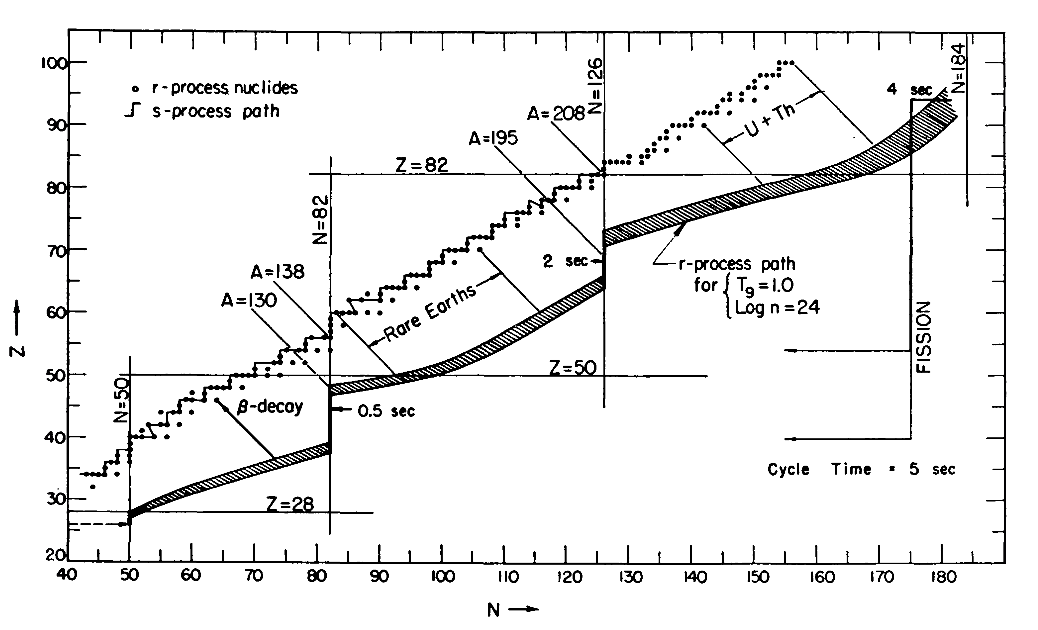
\includegraphics[height=8cm]{RProcessPath}
\caption{Nuclear chart of proton number against neutron number. At magic (shell closure) numbers, the r-process turns towards the line of stability and ``waits" for $\beta$ decay\cite{seeger}{}.}
\end{figure}

With knowledge of the path by which the r-process proceeds, and various experimental data such as reaction cross-sections and nuclei mass,  it is then possible to calculate the abundances of stable nuclides that should be observed in the universe\cite{seeger}{}.

\subsection{Proton Knockout}
In this project, properties of exotic, neutron rich nuclei far from stability have (hopefully) been measured. These nuclei have been accessed by proton knockout: the process by which protons knocked out of the nucleus by some incident particle. Though there are many different techniques for knockout reactions, the data analysed here come from experiments which have used real, polarised photons as the probe particle. 

Using photons is advantageous, as their interaction with the nucleus is purely electromagnetic, and so can be well determined using Quantum Electrodynamics (QED). Photons are unlikely to be perturbed by the nucleus as they approach, and are also unlikely to just be absorbed at the nuclear surface, allowing the entire nuclear volume to be probed\cite{robinson}{}. However, photo-reaction cross sections tend to be very small when compared with hadronic probes, as the electromagnetic interaction is relatively weak\cite{robinson}{}.

The wavelength of the photon determines the size of structure that it will interact with. As the energy of a photon is related to its wavelength by $E=\frac{hc}{\lambda}$, where $h$ and $c$ are Planck's constant and the speed of light respectively, it is thus the energy of the photon which is important. The cross-section for photon absorption depends on a number of different reaction mechanism contributions, which come in to play in different energy ranges. For example at low energies of $\sim30MeV$, the wavelength of a photon is such that it can couple to the entire nucleus as a whole, a phenomenon known as the giant dipole resonance. At higher energies of around $\sim300MeV$, the wavelength of a photon is sufficiently small to probe the constituent quarks of nucleons, leading to observations of the $\Delta$-resonance as individual nucleons are promoted to excited states.

Agreement is currently lacking as to the relative importance of the mechanisms which contribute to the single proton knockout reaction, $(\gamma,p)$\cite{meucci}{}. Some evidence points towards a mainly single step, direct knockout mechanism in which the photon interacts directly with the knocked-out nucleon\cite{boffi}{}. Experiments using polarisation-tagged photon beams however, indicate that a more prominent role is played by complex, multi-step mechanisms such as Meson Exchange Currents (MEC)\cite{bobeldijk}{}. Nuclear force is transmitted between nucleons by exchange of mesons, with the lightest $\pi$-mesons being particularly important for long-range (1-1.5fm) attraction between nucleons\cite{anwar}{}.
This leads to correlations between different nucleons, which can become important for how nucleon knockouts proceed.

MECs are also important in two proton knockout reactions, $(\gamma,pp)$, along with isobar currents, where the nucleons become excited, and direct knockout of correlated pairs. Numerous mechanisms make different contributions to the knockout cross section, depending on factors such as the energy regime\cite{robinson}{}. The number of coincident protons knocked out in a single reaction is determined here, and reaches up to (9). An understanding of the mechanisms leading to such reactions is currently lacking.

\subsection{The Crystal Ball at MAMI}
The Crystal Ball detector is an array of 672 NaI(Tl) crystals, capable of event detection over a solid angle of approximately $94\%$ of $4\pi sr$ ~\cite{tarbert}{}. The ball consists of two hermetically sealed hemispheres, which are evacuated in order to protect the hygroscopic detector crystals. The hemispheres meet at two $0.76mm$ steel plates, with a $5mm$ air gap in between, which reduces the detector acceptance by approximately $1.6\%$ ~\cite{starostin}{}. A further acceptance reduction of $6.7\%$ results from the gaps left for the beam entrance and exit tunnels, which occupy the space of 48 detector crystals. The interior radius of the ball is $25.3cm$, while the outer radius is $66.0cm$.

Targets are placed in the centre of the ball within a rohacell structural foam target holder\cite{tarbertThesis}{}. In turn, the target holder is situated within an evacuated carbon fibre pipe, sealed at one end with a kapton window.

Particle identification is performed by the Particle Identification Detector (PID), a $30cm$ long plastic barrel scintillator. Charged particles are distinguished based on specific ionisation energy loss, with energies deposited in the PID and Crystal Ball being correlated\cite{tarbertThesis}{}.

The PID is surrounded by a pair of multi wire proportional chambers, which consist of Tungsten wires running parallel to the beam axis sandwiched between aluminium laminated rohacell. The chambers are filled with a mixture of Argon, ethane, and freon gas and provide improved angular resolution for charged particles\cite{tarbertThesis}{}.

The photons beam used is produced by bremstrahlung using a metal foil radiator\cite{watts}{}. Electrons are directed at the radiator, and a fraction of the incident electrons undergo the photon producing bremstrahlung process\cite{tarbertThesis}{} $e^{-}+N \rightarrow e^{-}+N+\gamma$. This occurs when electrons experience an acceleration, as a result of the Couloumb field of the metal. The electron beam facility at MAMI uses three linear accelerator (LINAC) sections, followed by three race track microtrons to produce a beam of electrons with a duty factor of $\sim100$. A high duty factor means that particles arrive uniformly distributed in time, rather than in pulses\cite{wiedemann}{}. As a result of the high duty factor, a high intensity photon beam of $\sim10^{8} \gamma sec^{-1}$ can be produced. Scattered bremstrahulung electrons are momentum analysed using the Glasgow Tagger\cite{anthonyTagger}{}, which allows for determination of the bremstrahlung photon energies\cite{watts}{}.

%------- Literature Review begins -------------------------
\section{Literature Review}

Work on determining the abundances of chemical elements began, far removed from nuclear physics, in the field of geochemistry in the late 1800s\cite{clarke}. Using basic analysis, estimates were made of the abundance of chemical elements in the Earth's crust. Studies of meteorites paved the way for better estimates of the average abundances of elements in nature, rather than just on Earth, leading to a classic paper in 1937\cite{goldschmidt}{}. This acted as a springboard for much of what followed, and by 1956, the underlying nuclear physics processes that might have been responsible for the observed abundances were being considered\cite{suess}{}. In probably the most important paper in nuclear astrophysics, a comprehensive treatment of nucleosynthesis mechanisms, including the r-process, was published in 1957\cite{b2fh}{}. This laid out all of the key nucleosynthesis processes and analysed them within the context of a coherent framework, the theory of stellar nucleosynthesis. For this, as well as other contributions to astrophysics, one of the paper's authors was awarded the Nobel prize. Calculations of element abundances using the r-process were conducted in 1965\cite{seeger}{}, though then, as now, the lack of empirical data greatly affected accuracy. Since the 1960s, there has been little progress made in further advancing the conceptual understanding of the r-process. The precision of certain model parameters has been improved upon however, with much more now being known about exotic nuclei\cite{moller}{}. In spite of this, the problem remains that calculated r-process abundances do not agree with the observed abundances.

In the last decade, a new generation of radioactive ion beam facilities has been able to access the required nuclei, and experimental data such as $\beta$-decay half-lives of exotic nuclei are now becoming more available\cite{hosmer}{}$^{,}$\cite{lorusso}{}. Accessing exotic nuclei via photon-induced proton knockout has not been seriously attempted previously, and as such, much of the physics of knockout of more than two protons is currently unknown.

***Possible cut (
Photo-disintegration of an atomic nucleus was first observed in 1934, when high energy gamma rays were used to cause disintegration of a deuteron\cite{chadwick}{}. Although this landmark experiment is known for the  determination of the mass of the newly discovered neutron, it also stimulated interest in photon induced, `photonuclear' reactions. In the same year, neutrons were detected from a beryllium nucleus excited with gamma rays\cite{szilard}{}.

The advent of the synchrotron accelerator in the late 1940s facilitated several studies which observed protons and neutrons being emitted from nuclei that had been struck by high energy bremstrahlung photons\cite{perlman}\textsuperscript{,}\cite{levinthal}{}.It was predicted using a quasideuteron model that proton-neutron photo-pairs should be emitted in coincidence\cite{Levinger}{}. Further theoretical treatment of the direct interaction resulting in photo-nucleon emission soon followed\cite{gottfried}{}. A raft of further experiments with photons produced by continuous bremstrahlung supported the quasideuteron model\cite{smith}{}. Observations were also made of proton-proton, rather than proton-neutron knockout coincidences\cite{weinstein}{}.

In spite of the number of experiments, few real advances were made in understanding the reaction mechanisms that governed the photonucleon knockouts. As with the synchrotron decades before, the introduction of photon tagging at high duty factor beam facilities such as MAMI during the 1980s\cite{anthony} lead to something of a nuclear Renaissance. Within five years, angular and energy resolutions were sufficient to determine the shell that photo-nucleons had been knocked out of\cite{dancer}{}. In 1992, a microscopic model of how individual mechanisms contribute to nucleon knockout was published; the so-called Valencia model\cite{valencia}{}. Photon induced nucleon knockout reactions have since become a vital tool in the understanding of inter-nucleon interactions, such as short-range correlations between nucleons\cite{giusti}{}.
)***

\section{Method}
In order to calculate the mass of the residual nucleus after proton knockout, a missing mass reconstruction was employed. Essentially, this method utilises basic relativistic conservation of four-momentum. If the Lorentz vectors of the incoming photon beam and the initial state target are known, and those of the knocked out protons can be measured, then the ``missing" mass of the final state residual nucleus can be determined according to (\ref{eq:missingMass}).

\begin{equation}
\label{eq:missingMass}
M_{Missing} = (P_{Beam} + P_{Target} - \sum\limits_{i=1}^{N} P_{i} )^{2}
\end{equation}

Where in (\ref{eq:missingMass}), $M_{Missing}$ is the missing mass, the mass of the residual nucleus in this case, $P_{Beam}$ and $P_{Target}$ are the Lorentz vectors of the beam and target, and the sum is the sum of the Lorentz vectors of the $N$ knocked out protons.

However, before the data could be analysed, it was first necessary to calibrate the proton energies measured in the Crystal Ball.

\subsection{Energy Loss Calibration}
Proton energies measured in the Crystal Ball detectors are not the true values, and must be corrected for energy losses from several sources. Firstly, knocked out protons must escape the target, which causes them to lose energy. This is especially important in the case of lead, due to its high stopping power, but is significant for all target materials. Any material within the Crystal Ball also contributes to particle energies losses, for instance the PID and beam pipe lie in the path of the protons. Finally, energy loss in the NaI detector crystals due to light attenuation must be corrected for. 

The ionisation/excitation energy losses in the materials were simulated using the Geant4 simulation toolkit. Geant4 uses Monte-Carlo techniques for ``simulation of the passage of particles through matter"\cite{geant4}{}. The simulation geometry borrowed heavily from the setup developed at the University of Edinburgh for the A2 Collaboration\cite{lorenzo}{}. Protons were generated isotropically from the centre of the target with a given vertex energy. By comparing the energy at the detector with the initial vertex energy, it was possible to determine the energy loss of the protons. This was used to determine required angular cuts to the data. Energy loss is strongly dependent on the angle $\theta$, primarily as this determines what thickness of target the protons must escape from. Certain angles could also be cut, for instance the ``straight-through" angles on the beam axis, where the Crystal Ball does not have detectors, and angles where the protons must traverse particular support structures. Only protons detected within $22-76^{\circ}$ considered, as well as those within the same region plus $180^{\circ}$ due to the $\theta$ symmetry of the detector geometry. A study of the dependence of energy loss on $\phi$ was also conducted. Although there is a slight $\phi$ dependence with a periodic nature repeating over $7^{\circ}$ due to the fact that the PID is actually a polygon rather than a cylinder, this was not taken into account. The statistics of the $\theta$ study lead to an error $\sim 2\%$, and the $\phi$ variation in energy loss was deemed sufficiently small as to be negligible in comparison.

Once the cuts had been identified, the simulation was run at a single angle $\theta$, with protons being generated with random energies between $30-50MeV$. This was repeated in $2^{\circ}$ increments in $\theta$ using a million events per run.


\clearpage
\begin{thebibliography}{99}
%--------------- Introduction begins --------------------------------------
%--------------------------------------------------------------------------
\bibitem{cowan} Cowan, J.J. \& Thielemann, F.-K. ``R-Process Nucleosynthesis in Supernovae", \textit{Physics Today} \textbf{57}, pp 47 (2004).
%--------------------------------------------------------------------------
\bibitem{otsuka} Otsuka, T. ``Exotic nuclei and nuclear forces", \textit{Physica Srcipta} \textbf{2013}, T152 (2013).
%------------------------------------------------------------------------
\bibitem{thielemann} Thielemann, F.-K. et al. ``What are the astrophysical sites for the r-process and the production of heavy elements?", \textit{Progress in Particle and Nuclear Physics} \textbf{66}, pp346 (2011).
%--------------------------------------------------------------------------
%---------------- Introduction ends ----------------------------------------

%---------------- Background begins -----------------------------------------
%-----------------------------------------------------------------------------
\bibitem{iliadis} Iliadis, C. ``Nuclear Physics of Stars", 2nd Ed., Weinheim, Germany : Wiley-VCH Verlag GmbH \& Co. KGaA (2015).
%---------------------------------------------------------------------------
\bibitem{b2fh} Burbidge, E.M., Burbidge, G.R., Fowler, W.A., Hoyle, F. ``Synthesis of the Elements in Stars", \textit{Rev. Mod. Phys} \textbf{29}, pp547 (1957).
%------------------------------------------------------------------------------
\bibitem{warner} Warner, D. ``Not-so-magic numbers", \textit{Nature} \textbf{430}, pp517 (2004).
%-----------------------------------------------------------------------------
\bibitem{seeger} Seeger, P.A., Fowler, W.A., Clayton, D.D. ``Nucleosythesis of heavy elements by neutron capture", \textit{Astrophys. J. Suppl.} \textbf{11}, pp121 (1965).
%-----------------------------------------------------------------------------
\bibitem{robinson} Robinson, J. ``Two Proton Knockout From Carbon Using Linearly Polarized Photons", PhD Thesis, University of Glasgow (2010).
%-----------------------------------------------------------------------------
\bibitem{meucci} Meucci, A., Giusti, C., Pacati, F.D. ``Meson exchange currents in a relativistic model for electromagnetic one nucleon emission", \textit{Phys. Rev. C} \textbf{66}, 034610 (2002).
%------------------------------------------------------------------------------
\bibitem{boffi} Boffi, S., Giusti, C., Pacati, F.D. ``Direct nucleon emission by polarised photons", \textit{Nucl. Phys. A} \textbf{358}, 271c (1981).
%------------------------------------------------------------------------------
\bibitem{bobeldijk} Bobeldijk, I. et al. "Photon induced proton knockout from $^{208}$Pb", \textit{Phys. Lett. B} \textbf{356}, pp13 (1995). 
%------------------------------------------------------------------------------
\bibitem{anwar} Anwar, K. ``Nuclear Physics", Berlin : Springer (2014).
%----------------------------------------------------------------------------------
\bibitem{tarbert} Tarbert, C.M. et al. ``Incoherent Neutral Pion Photoproduction on $^{12}$C", \textit{Phys. Rev. Lett.} \textbf{100}, 132301 (2008).
%-----------------------------------------------------------------------------
\bibitem{starostin} Starostin, A. et al. ``Measurement of $K^{-}p \rightarrow \eta \Lambda$ near threshold", \textit{Phys. Rev. C} \textbf{64}, 055205 (2001).
%------------------------------------------------------------------------------
\bibitem{tarbertThesis} Tarbert, C.M. ``Coherent $\pi^{0}$ Photoproduction On Nuclei", PhD Thesis, University of Edinburgh (2007).
%----------------------------------------------------------------------------
\bibitem{watts} Watts, D.P. ``The Crystal Ball At MAMI" NSTAR 2005:Proceedings of the Workshop on the Physics of Excited Nucleons : Florida State University, Tallahassee, USA, 12-15 October 2005, Singapore : World Scientific, pp165 (2006).
%-----------------------------------------------------------------------------
\bibitem{wiedemann} Wiedermann, H. ``Particle Accelerator Physics", 4th Ed., Cham, Switzerland : Springer (2015).
%-----------------------------------------------------------------------------
\bibitem{anthonyTagger} Anthony, I., Kellie, J.D., Hall, S.J., Miller, G.J., Ahrens, J. ``Design of a tagged photon spectrometer for use with the Mainz 840 MeV microtron", \textit{Nucl. Instr. and Meth.} \textbf{301}, pp230 (1991).
%---------------------------------------------------------------------------
%--------------- Background Ends ---------------------------------------------
%--------------- Literature Review begins -----------------------------------
%----------------------------------------------------------------------------
\bibitem{clarke} Clarke, F.W. ``The relative abundances of the chemical elements", \textit{Bull. Phil. Soc. Washington} \textbf{11}, pp131 (1889).
%-----------------------------------------------------------------------------
\bibitem{goldschmidt} Goldschmidt, V.M. ``The Principles Of Distribution Of Chemical Elements In Minerals And Rocks : The Seventh Hugo Miller Lecture Delivered Before The Chemical Society On March 17th 1937", \textit{Journal of the Chemical Society (Resumed)} \textit{0}, pp655 (1937).
%-----------------------------------------------------------------------------
\bibitem{suess} Suess, H.E., Urey, H.C. ``Abundances of the Elements", \textit{Rev. Mod. Phys.} \textit{28}, pp53 (1956).
%----------------------------------------------------------------------------
\bibitem{moller} M\"oller, P., Nix, J.R., Kratz, K.-L. ``NUCLEAR PROPERTIES FOR ASTROPHYSICAL AND RADIOACTIVE-ION-BEAM APPLICATIONS", \textit{Atomic Data And Nuclear Data Tables} \textbf{66}, pp131 (1997).
\bibitem{chadwick} Chadwick, A. \& Goldhaber, M.``A `Nuclear Photo-effect': Disintegration of the Diplon by $\gamma$-Rays", \textit{Nature} \textbf{134}, pp237 (1934).
%----------------------------------------------------------------------------
\bibitem{hosmer} Hosmer, P. et al. ``Half-lives and branchings for $\beta$-delayed neutron emission for neutron-rich Co–Cu isotopes in the r-process", \textit{Phys. Rev. C} \textbf{82}, 025806 (2010).
%----------------------------------------------------------------------------
\bibitem{lorusso} Lorusso, G. et al. ``$\beta$-Decay Half-Lives of 110 Neutron-Rich Nuclei across the $N=82$ Shell Gap: Implications for the Mechanism and Universality of the Astrophysical r Process", \textit{Phys. Rev. Lett.} \textbf{114}, 192501 (2015).
%------------------------------------------------------------------------------
\bibitem{szilard} Szilard, L. \& Chalmers, T.A. ``Detection of Neutrons Liberated from Beryllium by Gamma Rays: a New Technique for Inducing Radioactivity", \textit{Nature} \textbf{134}, pp494 (1934).
%----------------------------------------------------------------------------
\bibitem{perlman} Perlman, M.L. \& Friedlander, G. ``Relative Yields of Some X-Ray Induced Nuclear Reactions", \textit{Phys. Rev.} \textbf{74}, pp442 (1948).
%----------------------------------------------------------------------------
\bibitem{levinthal} Levinthal, C. \& Silverman, A. ``Production of Protons by High Energy T-Rays", \textit{Phys. Rev.} \textbf{82}, pp822 (1951).
%----------------------------------------------------------------------------
\bibitem{Levinger} Levinger, J.S. ``The High Energy Nuclear Photoeffect", \textit{Phys. Rev.} \textbf{84}, pp43 (1951).
%----------------------------------------------------------------------------
\bibitem{gottfried} Gottfried, K. ``On The Determination Of The Nuclear Pair Correlation Function From The High Energy Photo-Effect", \textit{Nuclear Physics} \textbf{5}, pp557 (1958).
%-----------------------------------------------------------------------------
\bibitem{smith} Smith, I.L et al. ``The quasi-deuteron photodisintegration process in lithium,
carbon and calcium", \textit{Nuclear Physics B} \textbf{1}, pp483 (1967).
%------------------------------------------------------------------------------
\bibitem{weinstein} Weinstein, R.M. et al. ``Photoproton-Proton Coincidences From Various Nuclei", \textit{Phys. Rev.} \textbf{99}, pp1621 (1955).
%------------------------------------------------------------------------------
\bibitem{anthony} Anthony, I. et al. ``A Tagged Photon Spectrometer For The Mainz 180 MeV Microtron", \textit{Nuclear Physics A} \textbf{446}, pp321 (1985).
%------------------------------------------------------------------------------
\bibitem{dancer} Dancer, S.N. et al. ``Investigation of the \textsuperscript{12}C($\gamma$,pn) Reaction Using Tagged Photons", \textit{Phys. Rev. Lett.} \textbf{61}, pp1170 (1988).
%-----------------------------------------------------------------------------
\bibitem{valencia} Carrasco, R.C. \& Oset, E. ``Interaction Of Real Photons With Nuclei From 100 to 500MeV", \textit{Nuclear Physics A} \textbf{536}, pp445 (1992).
%-----------------------------------------------------------------------------
\bibitem{giusti} Giusti, C. \& Pacati, F.D. ``Photon-induced two-nucleon knockout reactions to discrete final states", \textit{Nuclear Physics A} \textbf{641}, pp297 (1998).
%----------------------- Literature Review ends -------------------------------
%----------------------- Method begins ----------------------------------------
\bibitem{geant4} Agostinelli, S. et al. ``Geant4 - a simulation toolkit", \textit{Nuclear Instruments and Methods in Physics Research Section A: Accelerators, Spectrometers, Detectors and Associated Equipment} \textbf{506}, pp250 (2003).
%------------------------------------------------------------------------------
\bibitem{lorenzo} Please see \url{http://www2.ph.ed.ac.uk/nuclear/G4/} for more information.

\end{thebibliography}
\end{document}